\begin{figure}[htbp]
\centering
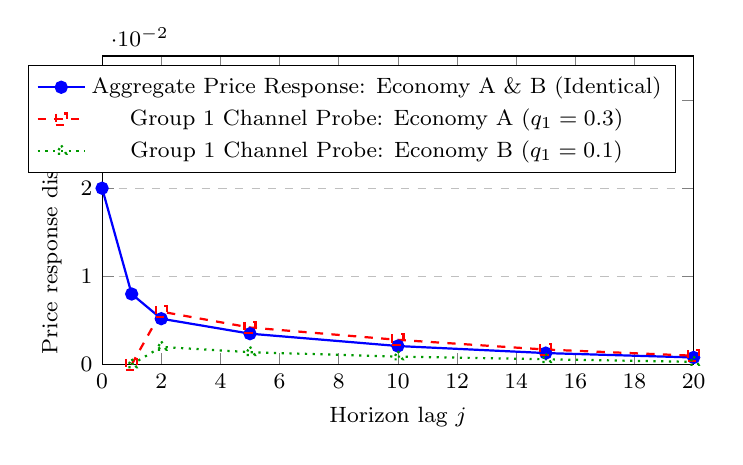
\begin{tikzpicture}
\begin{axis}[
    width=0.75\textwidth,
    height=5.5cm,
    xlabel={Horizon lag $j$},
    ylabel={Price response displacement},
    xmin=0, xmax=20,
    ymin=0, ymax=0.035,
    legend pos=north east,
    ymajorgrids=true,
    grid style=dashed,
    font=\footnotesize
]
\addplot[color=blue, mark=*, thick] coordinates {
    (0, 0.02) (1, 0.008) (2, 0.0052) (5, 0.0035) (10, 0.0021) (15, 0.0013) (20, 0.0008)
};
\addlegendentry{Aggregate Price Response: Economy A \& B (Identical)}

\addplot[color=red, mark=square, thick, dashed] coordinates {
    (1, 0.0) (2, 0.006) (5, 0.0042) (10, 0.0028) (15, 0.0017) (20, 0.0010)
};
\addlegendentry{Group 1 Channel Probe: Economy A ($q_1=0.3$)}

\addplot[color=green!60!black, mark=triangle, thick, dotted] coordinates {
    (1, 0.0) (2, 0.002) (5, 0.0014) (10, 0.0009) (15, 0.0006) (20, 0.0003)
};
\addlegendentry{Group 1 Channel Probe: Economy B ($q_1=0.1$)}
\end{axis}
\end{tikzpicture}
\caption{Group attribution under Proposition~G.1: identical aggregate price impulse responses vs.\ $3\times$ separation under group-specific channel probing.}
\label{fig:F4_group_attribution}
\end{figure}
